\let\negmedspace\undefined
\let\negthickspace\undefined
\documentclass[journal]{IEEEtran}
\usepackage[a5paper, margin=10mm, onecolumn]{geometry}
%\usepackage{lmodern} % Ensure lmodern is loaded for pdflatex
\usepackage{tfrupee} % Include tfrupee package

\setlength{\headheight}{1cm} % Set the height of the header box
\setlength{\headsep}{0mm}     % Set the distance between the header box and the top of the text

\usepackage{gvv-book}
\usepackage{gvv}
\usepackage{cite}
\usepackage{amsmath,amssymb,amsfonts,amsthm}
\usepackage{algorithmic}
\usepackage{graphicx}
\usepackage{textcomp}
\usepackage{xcolor}
\usepackage{txfonts}
\usepackage{listings}
\usepackage{enumitem}
\usepackage{mathtools}
\usepackage{gensymb}
\usepackage[breaklinks=true]{hyperref}
\usepackage{tkz-euclide} 
\usepackage{listings}
% \usepackage{gvv}                                        
\def\inputGnumericTable{}                                 
\usepackage[latin1]{inputenc}                                
\usepackage{color}                                            
\usepackage{array}                                            
\usepackage{longtable}                                       
\usepackage{calc}                                             
\usepackage{multirow}                                         
\usepackage{hhline}                                           
\usepackage{ifthen}                                           
\usepackage{lscape}
\usepackage{circuitikz}
\usepackage{comment}
\tikzstyle{block} = [rectangle, draw, fill=blue!20, 
    text width=4em, text centered, rounded corners, minimum height=3em]
\tikzstyle{sum} = [draw, fill=blue!10, circle, minimum size=1cm, node distance=1.5cm]
\tikzstyle{input} = [coordinate]
\tikzstyle{output} = [coordinate]


\begin{document}

\bibliographystyle{IEEEtran}
\vspace{3cm}

\title{10.4.2}
\author{EE25BTECH11026-Harsha}
 \maketitle
% \newpage
% \bigskip
{\let\newpage\relax\maketitle}

\renewcommand{\thefigure}{\theenumi}
\renewcommand{\thetable}{\theenumi}
\setlength{\intextsep}{10pt} % Space between text and floats


\numberwithin{equation}{enumi}
\numberwithin{figure}{enumi}
\renewcommand{\thetable}{\theenumi}

\textbf{Question}:\\
Find the equations of tangent and normal to the curve $y=\frac{x-7}{\brak{x-2}\brak{x-3}}$ at the point where it cuts the X axis.\\
\solution \\
Let us solve the given question theoretically and then verify the solution computationally.\\
\\
It is given that the tangents and normal are drawn at the point where the curve intersects the X axis i.e, at $\vec{P}=\myvec{7\\0}$ 
Let the equations of tangent be,
\begin{align}
    \vec{n_1}^{\top}\vec{x}=c_1 \label{eq:1}
\end{align}
And equation of normal be,
\begin{align}
    \vec{n_2}^{\top}\vec{x}=c_2 \label{eq:2}
\end{align}
To solve for their direction vectors, we can use he Jacobian technique.
It states that,
\begin{align}
    \vec{n}=\myvec{\frac{\partial{F}}{\partial{x}}\\\frac{\partial{F}}{\partial{y}}}_{\text{at point of tangency}}
\end{align}
where,
\begin{align*}
    \vec{n}:\text{Direction vector of tangent}\\
    \vec{F(x,y)}:\text{Function of the curve}
\end{align*}
Equation of the curve can be modified and written as,
\begin{align}
    yx^2-5xy+6y-x+7=0
\end{align}
\begin{align}
    \implies \vec{n}=\myvec{2xy-5y-1\\x^2-5x+6}
\end{align}
Substituting the point $\vec{P}$,
\begin{align}
    \therefore \vec{n_1}=\myvec{-1\\20} \label{eq:3}
\end{align}
\begin{align}
    \implies \vec{n_2}=\myvec{20\\1} \label{eq:4}
\end{align}
\newpage
\vspace*{0.25cm}
Substituing ~\eqref{eq:3} and ~\eqref{eq:4} in ~\eqref{eq:1} and ~\eqref{eq:2} respectively yields,
\begin{align}
    \myvec{-1&&20}\vec{x}=c_1 \label{eq:5} \\
    \myvec{20&&1}\vec{x}=c_2 \label{eq:6}
\end{align}
Substituting $\vec{P}$ in ~\eqref{eq:5} and ~\eqref{eq:6},
\begin{align}
    \implies c_1=-7 \quad and \quad c_2=140
\end{align}
\begin{align}
    \therefore \text{Equation of tangent:} \myvec{-1&&20}\vec{x}=-7
\end{align}
\begin{align}
    \therefore \text{Equation of normal:} \myvec{20&&1}\vec{x}=140
\end{align}

From the figure, it is clearly verified that the theoretical solution matches with the computational solution.\\

\begin{figure}[H]
    \centering
    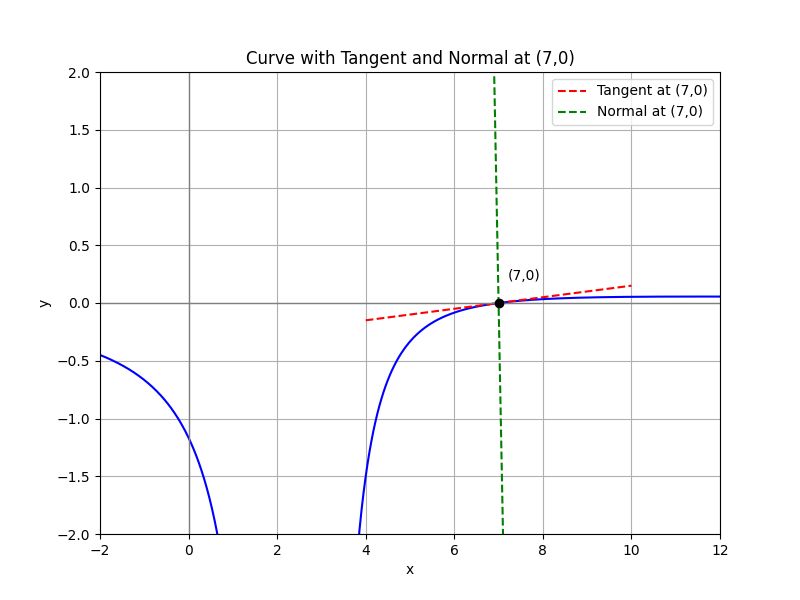
\includegraphics[width=0.8\columnwidth]{figs/Figure_1.png}
    \label{fig:1}
\end{figure}

\end{document}
